% homework/hw08x/hw08x.tex
% Year 7 - Extra Homework: the point never moves.
%
% Goes out alongside Homework 8. Same framing rule as hw03x through hw07x:
% nothing on the sheet says easy, basic, extra help, catch-up or revision, and
% no question is marked as being for anybody in particular. The cover states a
% fact, and it is a true one:
%
%   4.6, 46, 460 and 0.46 are the same two digits. What tells you which number
%   you are looking at is WHERE THE POINT IS.
%
% THAT IS THE WHOLE DESIGN. Every question on the sheet is the same two or
% three digits standing somewhere else, so "multiply by 100" stops being a rule
% to remember and becomes a thing you can watch happen in a place-value table.
% The folk rule the deck kills on slide 8 -- "to multiply by 10, add a zero" --
% cannot survive a table, because you can see the digits move and the point
% stay.
%
% QUESTION NUMBERS ARE X1..X20, NOT F1..F20. Homework 8 has a Section F of its
% own (F1, F2, F3) and the two sheets go home in the same envelope, so "F2"
% would name two different questions on the same evening.
%
% Part 4 is here on purpose. The mass ladder came out of Homework 8 (it was
% E2) for the page target, and mg/g/kg/t is a stated objective of 3.1, so it
% had to land somewhere. It lands here, at length, with the ladder drawn.
%
% X20 is the sheet in miniature and the last question on purpose: 0.045 kg is
% 45 g is 45000 mg, and the digits 4 and 5 never change. Only where the point
% is.
%
% House style is shared: see homework/hw-style.tex. Method: the new-homework
% skill. Source is pure ASCII on purpose.
%
% Build:  pwsh .claude/skills/new-homework/scripts/build-hw.ps1 hw08x

\documentclass[12pt,a4paper]{article}

% -- Answer key switch -------------------------------------------------------
\newif\ifkey
\ifdefined\TEACHER\keytrue\else
  \keyfalse        % \keyfalse = student copy   |   \keytrue = teacher copy
\fi

% -- House style -------------------------------------------------------------
% homework/hw-style.tex
% Shared house style for every Year 7 homework packet. \input this from the
% packet file, right after \documentclass and the answer-key switch.
%
% Do not fork this file per packet. If a packet needs a different look, the
% question is whether every packet should have it.
%
% The choices here are deliberate and were arrived at by printing and looking:
%   * No solid dark banners. Every header is a light tint with a coloured spine
%     on the left, so colour reads clearly without flooding a school printer.
%   * No marks and no mark totals. These are practice, not exam papers.
%   * Lato at 12pt with open leading, plus mathastext so inline maths is Lato
%     too. Without mathastext every "-6 + 4" is Computer Modern serif and the
%     sheet looks half-typeset.
%   * Writing lines are spaced for Year 7 handwriting, not adult margin notes.
%
% Provides: \wlines \blank \tickbox \sep \qmk-free marks (none) \hwsection
% \qhead \expr, the workspace box, and the remember / wordhelp / activity /
% yourturn coloured boxes. Palette matches the lesson decks exactly.

% -- Packages ----------------------------------------------------------------
\usepackage[T1]{fontenc}
\usepackage[utf8]{inputenc}
\usepackage[default]{lato}
\usepackage[a4paper,top=1.7cm,bottom=1.7cm,left=2.0cm,right=2.0cm,headheight=15pt]{geometry}
\usepackage{amsmath,amssymb}
\usepackage{xcolor}
\usepackage[most]{tcolorbox}
\usepackage{enumitem}
\usepackage{tikz}
\usetikzlibrary{arrows.meta}
\usepackage{array}
\usepackage{tabularx}
\usepackage{fancyhdr}
\usepackage{multicol}
\usepackage{needspace}
\usepackage{graphicx}

% Make maths use Lato too. Without this, every "-6 + 4" on the page is set in
% Computer Modern serif and the sheet looks half-typeset. Must come last.
\usepackage[italic]{mathastext}

\linespread{1.06}\selectfont

% -- The Learner's Book palette (same hex values as the lesson decks) ---------
\definecolor{cbteal}{HTML}{0087A8}
\definecolor{cbpurple}{HTML}{5C2483}
\definecolor{cborange}{HTML}{C25E12}
\definecolor{cbgreen}{HTML}{4A8B23}
\definecolor{cbred}{HTML}{C8102E}
\definecolor{cbblue}{HTML}{1A5FA8}
\definecolor{rulegray}{HTML}{9AA5AD}

% -- Answer lines and blanks -------------------------------------------------
% \wlines{n} draws n ruled writing lines, spaced wide enough for Year 7
% handwriting rather than for an adult with a fine pen.
\makeatletter
\newcommand{\wlines}[1]{%
  \par\vspace{0.75em}%
  \@tempcnta=0\relax
  \@whilenum\@tempcnta<#1\do{%
    \hbox to \linewidth{\color{rulegray}\leaders\hrule height 0.5pt\hfill}%
    \vspace{1.5em}%
    \advance\@tempcnta by 1\relax}%
  \par\vspace{-0.8em}%
}
\makeatother

% \blank[width] is an inline gap to write a short answer in.
\newcommand{\blank}[1][2.6cm]{\underline{\hspace{#1}}}

% A boxed space for showing working.
\newtcolorbox{workspace}[1][3.4cm]{%
  colback=white, colframe=rulegray, boxrule=0.5pt, arc=5pt,
  height=#1, left=6pt, right=6pt, top=4pt, bottom=4pt,
  before skip=9pt, after skip=11pt}

% An empty tick box.
\newcommand{\tickbox}{\fbox{\rule{0pt}{1.15em}\rule{1.15em}{0pt}}}

% A middot separator.
\newcommand{\sep}{\,\textperiodcentered\,}

% -- Section and question headings -------------------------------------------
% Light tint plus a fat coloured spine on the left. No solid dark banner: the
% colour reads clearly but barely costs the printer anything.
% needspace stops a heading stranding alone at the foot of a page. Kept modest:
% too large and it pushes headings over, leaving a worse hole than it prevents.
\newcommand{\hwsection}[2][cbteal]{%
  \needspace{8\baselineskip}%
  \par\vspace{13pt}%
  \noindent
  \begin{tcolorbox}[enhanced, nobeforeafter, width=\textwidth,
      colback=#1!7, colframe=#1!7, arc=5pt,
      borderline west={5pt}{0pt}{#1},
      left=14pt, right=10pt, top=7pt, bottom=7pt]
    {\large\bfseries\color{#1}#2}
  \end{tcolorbox}%
  \par\vspace{9pt}}

% \qhead[colour]{A2}{Moving along the line} -- a question heading.
\newcommand{\qhead}[3][cbteal]{%
  \needspace{6\baselineskip}%
  \par\vspace{11pt}%
  \noindent{\large\bfseries\color{#1}#2}\quad{\large\bfseries #3}\par\vspace{4pt}}

% -- Coloured boxes ----------------------------------------------------------
% Shared look: rounded, light fill, coloured rule, coloured title text on a
% pale title strip rather than a dark one.
\tcbset{hwbox/.style={
  enhanced, breakable, arc=6pt, boxrule=1pt,
  left=11pt, right=11pt, top=8pt, bottom=8pt,
  fonttitle=\bfseries, attach boxed title to top left={xshift=12pt, yshift=-8pt},
  boxed title style={arc=4pt, boxrule=1pt, left=7pt, right=7pt, top=2pt, bottom=2pt},
  top=13pt}}

% Orange: things to remember. Matches the deck's "Write This Down".
\newtcolorbox{remember}[1][Remember from the lesson]{hwbox,
  colback=cborange!6, colframe=cborange, coltitle=cborange,
  colbacktitle=white, title={#1}}

% Blue: English help. The barrier in this class is the wording, not the maths.
\newtcolorbox{wordhelp}[1][Word help]{hwbox,
  colback=cbblue!6, colframe=cbblue, coltitle=cbblue,
  colbacktitle=white, title={#1}}

% Purple: an activity or instruction.
\newtcolorbox{activity}[1][How to do this homework]{hwbox,
  colback=cbpurple!6, colframe=cbpurple, coltitle=cbpurple,
  colbacktitle=white, title={#1}}

% Green: your turn / a friendly nudge.
\newtcolorbox{yourturn}[1][Your turn]{hwbox,
  colback=cbgreen!7, colframe=cbgreen, coltitle=cbgreen!75!black,
  colbacktitle=white, title={#1}}

% -- Shorthands --------------------------------------------------------------
\newcommand{\dC}{\,^{\circ}\mathrm{C}}          % use inside maths: $-8\dC$
\newcommand{\key}[1]{{\color{cborange}\textbf{#1}}}
\newcommand{\eng}[1]{{\color{cbblue}\textbf{#1}}}

\setlist[enumerate]{itemsep=8pt, topsep=5pt, leftmargin=*}
\setlist[itemize]{itemsep=4pt, topsep=4pt, leftmargin=*}
\renewcommand{\arraystretch}{1.45}

% -- An expression the student is asked to work from -------------------------
\newcommand{\expr}[1]{%
  \tcbox[on line, colback=cbgreen!10, colframe=cbgreen!55, boxrule=1pt, arc=4pt,
         left=9pt, right=9pt, top=4pt, bottom=4pt]{\large\bfseries $#1$}}

% -- Running head and foot ---------------------------------------------------
% The packet overrides \fancyhead[L] with its own title.
\pagestyle{fancy}
\fancyhf{}
\fancyhead[L]{\small\color{black!55}Year 7\sep Homework}
\fancyhead[R]{\small\color{black!55}Name: \blank[3.4cm]}
\fancyfoot[C]{\small\color{black!55}Page \thepage}
\renewcommand{\headrulewidth}{0pt}
\renewcommand{\headrule}{\vspace{2pt}\hbox to\headwidth{\color{cbteal!45}\leaders\hrule height 1.2pt\hfill}}



% -- Per-packet running head -------------------------------------------------
\fancyhead[L]{\small\color{black!55}Year 7\sep Extra Homework}

% -- A group of writing lines that will not be split -------------------------
\newcommand{\qlines}[1]{\par\needspace{\numexpr#1+1\relax\baselineskip}\wlines{#1}}

% -- A box to write one digit in ---------------------------------------------
% The workbook's own scaffold: a part-written line with an empty square where
% the digit goes. Filling the squares IS the method being taught, so it has to
% look like something you write in, not like a blank.
\newcommand{\nbox}{\ \fbox{\rule{0pt}{1.05em}\rule{1.0em}{0pt}}\ }

% -- An answer blank that will not cause an overfull line ---------------------
% "\hfill \blank[..]" at the end of a wrapping paragraph overflows the margin
% when the text happens to fill its last line: the blank has nowhere to go and
% hangs off the right edge. \ansline puts it on a line of its own,
% right-aligned, which cannot overflow whatever the text does.
\newcommand{\ansline}[1][4.4cm]{\par\vspace{2pt}\hspace*{\fill}\blank[#1]\par}

% -- A ragged-right X column -------------------------------------------------
\newcolumntype{L}{>{\raggedright\arraybackslash}X}

% -- A centred fixed-width column --------------------------------------------
\newcolumntype{C}[1]{>{\centering\arraybackslash}p{#1}}

% -- The place-value table ---------------------------------------------------
% Seven columns, with a narrow one in the middle for the point. The headings
% are words rather than fractions on purpose: tenths, hundredths and
% thousandths are the English being taught, and a student who cannot say them
% cannot read the question that uses them.
\newcommand{\pvhead}{%
  \textbf{hundreds} & \textbf{tens} & \textbf{ones} & \textbf{$\cdot$} &
  \textbf{tenths} & \textbf{hundredths} & \textbf{thousandths}}
\newenvironment{pvtable}{%
  \renewcommand{\arraystretch}{1.7}%
  \small
  \noindent
  \begin{tabular}{|C{1.9cm}|C{1.9cm}|C{1.9cm}|C{0.5cm}|C{1.9cm}|C{2.3cm}|C{2.5cm}|}
  \hline}
  {\end{tabular}\renewcommand{\arraystretch}{1.45}}

% -- A number line from one whole number to the next, marked in tenths -------
% #1 left label, #2 right label, #3 and #4 the two tenths to mark (0 to 10),
% given as integers so the \foreach and the tick positions agree.
\newcommand{\tenthline}[4]{%
  \begin{tikzpicture}[x=1.28cm, y=1cm, line width=0.9pt]
    \draw[cbteal] (-0.35,0) -- (10.35,0);
    \foreach \n in {0,...,10}{\draw[cbteal] (\n,-0.13) -- (\n,0.13);}
    \draw[cbteal, line width=1.6pt] (0,-0.22) -- (0,0.22);
    \draw[cbteal, line width=1.6pt] (10,-0.22) -- (10,0.22);
    \node[below=4pt, font=\small\bfseries] at (0,-0.22) {$#1$};
    \node[below=4pt, font=\small\bfseries] at (10,-0.22) {$#2$};
    \draw[cborange, line width=1.7pt] (#3,-0.30) -- (#3,0.30);
    \node[above=2pt, font=\small\bfseries, text=cborange] at (#3,0.30) {\textbf{P}};
    \draw[cbpurple, line width=1.7pt] (#4,-0.30) -- (#4,0.30);
    \node[above=2pt, font=\small\bfseries, text=cbpurple] at (#4,0.30) {\textbf{Q}};
  \end{tikzpicture}}

\begin{document}

% ===========================================================================
% COVER BLOCK
% ===========================================================================
\thispagestyle{fancy}

\begin{tcolorbox}[enhanced, colback=cbgreen!8, colframe=cbgreen!8, arc=7pt,
                  borderline west={6pt}{0pt}{cbgreen},
                  left=18pt, right=14pt, top=11pt, bottom=11pt]
  {\color{cbgreen!75!black}\bfseries YEAR 7\sep UNIT 3\sep EXTRA HOMEWORK}\\[6pt]
  {\color{cbgreen!70!black}\Huge\bfseries The Point Never Moves}\\[10pt]
  {\color{black!70}Reading decimals\sep multiplying and dividing by 10\sep rounding\sep mg, g, kg and t}
\end{tcolorbox}

\vspace{6pt}
\noindent
\begin{tabularx}{\textwidth}{@{}X X@{}}
  \textbf{Name:} \blank[5.6cm] & \textbf{Class:} \blank[5.6cm] \\
  \textbf{Date given:} \blank[4.6cm] &
  \textbf{Date due:} {\color{cbred}\bfseries Monday 28 September 2026} \\
\end{tabularx}

\vspace{4pt}
\begin{activity}[Why this sheet exists]
  \key{0.46}, \key{4.6}, \key{46} and \key{460} are the \key{same two digits}.
  Nothing about the 4 or the 6 is different. What tells you which number you are
  looking at is \key{where the point is}.

  \medskip
  So when somebody says ``multiply by 100'', the point \key{stays exactly where it
  is} and the \key{digits move} two columns to the left. That is why $7.2 \times
  10^3$ is $7200$ and not $7.2000$ --- and you can watch it happen in the tables
  on this sheet.

  \medskip
  \eng{No calculator.} Write in every box.
\end{activity}

% ===========================================================================
% PART 1 -- WHERE THE POINT IS
% ===========================================================================
\hwsection[cbgreen]{Part 1 \textperiodcentered\ Where the point is}

% -- X1 ---------------------------------------------------------------------
\qhead[cbgreen]{X1}{One digit per column}

\noindent Put each number into the table. One digit goes in each column. The first
one is done for you.

\vspace{6pt}
\begin{center}
\begin{pvtable}
  \pvhead \\ \hline
  \multicolumn{7}{|l|}{\rule{0pt}{1.6em}\textbf{47.3}} \\ \hline
  & 4 & 7 & $\cdot$ & 3 & & \\ \hline
  \multicolumn{7}{|l|}{\rule{0pt}{1.6em}\textbf{6.85}} \\ \hline
  & & & $\cdot$ & & & \\ \hline
  \multicolumn{7}{|l|}{\rule{0pt}{1.6em}\textbf{130.06}} \\ \hline
  & & & $\cdot$ & & & \\ \hline
  \multicolumn{7}{|l|}{\rule{0pt}{1.6em}\textbf{0.904}} \\ \hline
  & & & $\cdot$ & & & \\ \hline
\end{pvtable}
\end{center}

% -- X2 ---------------------------------------------------------------------
\qhead[cbgreen]{X2}{The same digit, five different jobs}

\noindent Every number below has a \textbf{6} in it, and the 6 is worth something
different every time. Join each number to what its 6 is worth. The first one is done
for you.

\begin{wordhelp}[Word help --- the columns after the point]
  \begin{tabularx}{\linewidth}{@{}l@{\hspace{16pt}}X@{}}
    \eng{tenths} & the \textbf{first} column after the point. $0.6$ is six tenths \\
    \eng{hundredths} & the \textbf{second} column. $0.06$ is six hundredths \\
    \eng{thousandths} & the \textbf{third} column. $0.006$ is six thousandths \\
  \end{tabularx}
\end{wordhelp}

\vspace{2pt}
\noindent
\begin{tabularx}{\textwidth}{|C{2.4cm}|c|L|}
  \hline
  \textbf{Number} & & \textbf{What the 6 is worth} \\
  \hline
  1.\ $6.2$ \rule[-0.6em]{0pt}{1.9em}   & \textbf{C} & \textbf{A} \; six tenths \\ \hline
  2.\ $0.63$ \rule[-0.6em]{0pt}{1.9em}  & \tickbox & \textbf{B} \; six hundredths \\ \hline
  3.\ $0.86$ \rule[-0.6em]{0pt}{1.9em}  & \tickbox & \textbf{C} \; six ones \\ \hline
  4.\ $0.006$ \rule[-0.6em]{0pt}{1.9em} & \tickbox & \textbf{D} \; six tens \\ \hline
  5.\ $62.5$ \rule[-0.6em]{0pt}{1.9em}  & \tickbox & \textbf{E} \; six thousandths \\ \hline
\end{tabularx}

% -- X3 ---------------------------------------------------------------------
% The English of reading a decimal out loud, which nothing else on either
% packet teaches and which decides half the marks in a listening task.
\qhead[cbgreen]{X3}{Saying it out loud}

\begin{remember}[After the point, one digit at a time]
  $12.34$ is \key{``twelve point three four''}. \;
  {\color{cbred}\bfseries Not ``twelve point thirty-four''.}

  \smallskip
  The digits after the point are read \key{one by one}, so a zero has to be said:
  $4.05$ is \key{``four point zero five''}.
\end{remember}

\vspace{2pt}
\noindent
\begin{tabularx}{\textwidth}{|C{2.4cm}|L|}
  \hline
  \textbf{Number} & \textbf{Say it} \\
  \hline
  $12.34$ \rule[-0.6em]{0pt}{1.9em} & twelve point three four \\ \hline
  $5.9$ \rule[-0.6em]{0pt}{1.9em}   & \\ \hline
  $0.71$ \rule[-0.6em]{0pt}{1.9em}  & \\ \hline
  $8.06$ \rule[-0.6em]{0pt}{1.9em}  & \\ \hline
  \rule[-0.6em]{0pt}{1.9em}         & three point one four \\ \hline
  \rule[-0.6em]{0pt}{1.9em}         & twenty point zero five \\ \hline
\end{tabularx}

% -- X4 ---------------------------------------------------------------------
\qhead[cbgreen]{X4}{Which is bigger?}

\noindent Write $<$ or $>$ in each box.

\begin{remember}[A longer number is not a bigger number]
  $0.65$ has more digits than $0.7$, and it is \key{smaller}. Compare the
  \key{tenths first}: 6 tenths against 7 tenths. \; So $0.65 < 0.7$.
\end{remember}

\vspace{2pt}
\begin{multicols}{3}
\begin{enumerate}[label=(\alph*), itemsep=11pt]
  \item $0.4 \;\nbox\; 0.35$
  \item $0.8 \;\nbox\; 0.81$
  \item $2.5 \;\nbox\; 2.45$
  \item $0.09 \;\nbox\; 0.1$
  \item $7.30 \;\nbox\; 7.3$
  \item $0.62 \;\nbox\; 0.6$
\end{enumerate}
\end{multicols}

\vspace{2pt}
\noindent One pair in that list is \textbf{neither} bigger nor smaller. Which one, and
why?
\ansline[8.0cm]

% ===========================================================================
% PART 2 -- MOVING THE DIGITS
% ===========================================================================
\hwsection[cbgreen]{Part 2 \textperiodcentered\ Moving the digits}

% -- X5 ---------------------------------------------------------------------
\qhead[cbgreen]{X5}{Watch it happen}

\noindent Each row is the row above it multiplied by \textbf{10}. Every digit moves
\textbf{one column to the left}. Fill in the rest of the table.

\vspace{6pt}
\begin{center}
\begin{pvtable}
  \pvhead \\ \hline
  \rule{0pt}{1.6em} & & 4 & $\cdot$ & 6 & & \\ \hline
  \rule{0pt}{1.6em} & 4 & 6 & $\cdot$ & & & \\ \hline
  \rule{0pt}{1.6em} & & & $\cdot$ & & & \\ \hline
\end{pvtable}
\end{center}

\vspace{6pt}
\noindent \textbf{(a)} Write the three numbers. \; $4.6$, \blank[2.4cm],
\blank[2.4cm]

\vspace{7pt}
\noindent \textbf{(b)} The 4 and the 6 are in all three rows. What moved, and what
stayed still?
\ansline[8.0cm]

% -- X6 ---------------------------------------------------------------------
\qhead[cbgreen]{X6}{Multiplying moves the digits left}

\noindent One place for 10, two for 100, three for 1000.

\vspace{4pt}
\begin{multicols}{3}
\begin{enumerate}[label=(\alph*), itemsep=11pt]
  \item $3.2 \times 10 = \blank[1.7cm]$
  \item $0.7 \times 10 = \blank[1.7cm]$
  \item $5.48 \times 10 = \blank[1.7cm]$
  \item $3.2 \times 100 = \blank[1.7cm]$
  \item $0.7 \times 100 = \blank[1.7cm]$
  \item $6.9 \times 100 = \blank[1.7cm]$
  \item $3.2 \times 1000 = \blank[1.7cm]$
  \item $0.05 \times 100 = \blank[1.7cm]$
  \item $1.28 \times 1000 = \blank[1.7cm]$
\end{enumerate}
\end{multicols}

% -- X7 ---------------------------------------------------------------------
\qhead[cbgreen]{X7}{Dividing moves the digits right}

\begin{remember}[The zeros you have to write yourself]
  $7 \div 100$. The 7 moves two columns right, past the ones and past the tenths,
  and lands in the \key{hundredths}. Nothing is left in the ones or the tenths, so
  you write \key{0} in both: \; $7 \div 100 = \mathbf{0.07}$.
\end{remember}

\vspace{2pt}
\begin{multicols}{3}
\begin{enumerate}[label=(\alph*), itemsep=11pt]
  \item $46 \div 10 = \blank[1.7cm]$
  \item $8 \div 10 = \blank[1.7cm]$
  \item $520 \div 10 = \blank[1.7cm]$
  \item $46 \div 100 = \blank[1.7cm]$
  \item $8 \div 100 = \blank[1.7cm]$
  \item $520 \div 100 = \blank[1.7cm]$
  \item $46 \div 1000 = \blank[1.7cm]$
  \item $9 \div 1000 = \blank[1.7cm]$
  \item $3.5 \div 100 = \blank[1.7cm]$
\end{enumerate}
\end{multicols}

% -- X8 ---------------------------------------------------------------------
\qhead[cbgreen]{X8}{The little raised number}

\begin{remember}[The power counts the zeros]
  $10^2$ means $10 \times 10 = 100$. Two zeros. \quad
  $10^3$ means $10 \times 10 \times 10 = 1000$. Three zeros.

  \smallskip
  Say it aloud: $10^2$ is \key{``ten squared''}, $10^3$ is \key{``ten cubed''},
  $10^4$ is \key{``ten to the power of four''}.
\end{remember}

\vspace{2pt}
\noindent
\begin{tabularx}{\textwidth}{|C{2.0cm}|C{2.4cm}|L|}
  \hline
  \textbf{Power} & \textbf{Written out} & \textbf{Say it} \\
  \hline
  $10^2$ \rule[-0.6em]{0pt}{1.9em} & 100 & ten squared \\ \hline
  $10^3$ \rule[-0.6em]{0pt}{1.9em} & & \\ \hline
  $10^5$ \rule[-0.6em]{0pt}{1.9em} & & \\ \hline
  \rule[-0.6em]{0pt}{1.9em} & 10\,000 & \\ \hline
\end{tabularx}

% -- X9 ---------------------------------------------------------------------
\qhead[cbgreen]{X9}{Now with the power written in}

\noindent Same job as X6 and X7. The power tells you \textbf{how many places}.

\begin{remember}[The folk rule is wrong]
  ``To multiply by 10, add a zero'' works for whole numbers and \key{nothing else}.
  \; $7.2 \times 10^3$ is \key{7200}. \;
  {\color{cbred}\bfseries Not 7.2000, which is just 7.2.}
\end{remember}

\vspace{2pt}
\begin{multicols}{2}
\begin{enumerate}[label=(\alph*), itemsep=11pt]
  \item $2.4 \times 10^2 = \blank[2.4cm]$
  \item $0.06 \times 10^3 = \blank[2.4cm]$
  \item $15 \times 10^4 = \blank[2.4cm]$
  \item $830 \div 10^2 = \blank[2.4cm]$
  \item $6 \div 10^3 = \blank[2.4cm]$
  \item $2.5 \div 10^1 = \blank[2.4cm]$
\end{enumerate}
\end{multicols}

% -- X10 --------------------------------------------------------------------
\qhead[cbgreen]{X10}{Which way, and how far?}

\noindent Look at what happened to the digits. Write \textbf{left} or \textbf{right},
and how many places. The first one is done for you.

\vspace{4pt}
\noindent
\begin{tabularx}{\textwidth}{|C{2.0cm}|C{0.8cm}|C{2.0cm}|C{2.6cm}|C{2.4cm}|L|}
  \hline
  \textbf{From} & & \textbf{To} & \textbf{Left or right?} & \textbf{How many places?}
  & \textbf{So you} \\
  \hline
  $4.8$ \rule[-0.6em]{0pt}{1.9em} & $\rightarrow$ & $480$ & left & 2 &
    $\times 10^2$ \\ \hline
  $6.1$ \rule[-0.6em]{0pt}{1.9em} & $\rightarrow$ & $0.061$ & & & \\ \hline
  $90$ \rule[-0.6em]{0pt}{1.9em}  & $\rightarrow$ & $9000$ & & & \\ \hline
  $7$ \rule[-0.6em]{0pt}{1.9em}   & $\rightarrow$ & $0.7$ & & & \\ \hline
\end{tabularx}

% ===========================================================================
% PART 3 -- STOPPING SOMEWHERE
% ===========================================================================
\hwsection[cbgreen]{Part 3 \textperiodcentered\ Stopping somewhere}

% -- X11 --------------------------------------------------------------------
\qhead[cbgreen]{X11}{Which end is it nearer?}

\noindent The line below runs from \textbf{3} to \textbf{4}, and it is marked in
\textbf{tenths}.

\vspace{6pt}
\begin{center}
\tenthline{3}{4}{4}{7}
\end{center}

\vspace{7pt}
\begin{enumerate}[label=(\alph*), itemsep=9pt]
  \item Write the number that \textbf{P} is marking. \hfill \blank[3.0cm]
  \item Write the number that \textbf{Q} is marking. \hfill \blank[3.0cm]
  \item Is \textbf{P} nearer to 3 or to 4? \hfill \blank[3.0cm]
  \item Is \textbf{Q} nearer to 3 or to 4? \hfill \blank[3.0cm]
\end{enumerate}

% -- X12 --------------------------------------------------------------------
\qhead[cbgreen]{X12}{Round to the nearest whole number}

\begin{remember}[Look at the next digit only]
  Look at the \key{tenths} digit. \; \textbf{0, 1, 2, 3, 4} --- round \key{down}.
  \; \textbf{5, 6, 7, 8, 9} --- round \key{up}.

  \smallskip
  \hspace*{1.2em}$12.3 \rightarrow \mathbf{12}$ \qquad
  $12.8 \rightarrow \mathbf{13}$ \qquad $12.5 \rightarrow \mathbf{13}$
\end{remember}

\vspace{2pt}
\begin{multicols}{3}
\begin{enumerate}[label=(\alph*), itemsep=11pt]
  \item $6.2 \rightarrow \blank[1.5cm]$
  \item $8.9 \rightarrow \blank[1.5cm]$
  \item $14.5 \rightarrow \blank[1.5cm]$
  \item $0.4 \rightarrow \blank[1.5cm]$
  \item $29.8 \rightarrow \blank[1.5cm]$
  \item $0.61 \rightarrow \blank[1.5cm]$
\end{enumerate}
\end{multicols}

% -- X13 --------------------------------------------------------------------
\qhead[cbgreen]{X13}{Counting decimal places}

\noindent \textbf{Decimal places} are the digits \textbf{after the point}. Start
counting \textbf{at the point}, not at the front of the number.

\vspace{4pt}
\noindent
\begin{tabularx}{\textwidth}{|C{2.4cm}|C{3.4cm}|C{2.4cm}|L|}
  \hline
  \textbf{Number} & \textbf{How many d.p.?} & \textbf{Number} &
  \textbf{How many d.p.?} \\
  \hline
  $5.28$ \rule[-0.6em]{0pt}{1.9em}    & 2 &
  $130.4$ \rule[-0.6em]{0pt}{1.9em}   & \\ \hline
  $0.9$ \rule[-0.6em]{0pt}{1.9em}     & &
  $7.0625$ \rule[-0.6em]{0pt}{1.9em}  & \\ \hline
  $12.346$ \rule[-0.6em]{0pt}{1.9em}  & &
  $86$ \rule[-0.6em]{0pt}{1.9em}      & \\ \hline
\end{tabularx}

% -- X14 --------------------------------------------------------------------
\qhead[cbgreen]{X14}{Round to 1 decimal place}

\noindent Keep \textbf{one} digit after the point. Look at the \textbf{second} digit
after the point to decide.

\vspace{4pt}
\begin{multicols}{3}
\begin{enumerate}[label=(\alph*), itemsep=11pt]
  \item $4.62 \rightarrow \blank[1.5cm]$
  \item $8.17 \rightarrow \blank[1.5cm]$
  \item $0.348 \rightarrow \blank[1.5cm]$
  \item $23.75 \rightarrow \blank[1.5cm]$
  \item $9.44 \rightarrow \blank[1.5cm]$
  \item $0.251 \rightarrow \blank[1.5cm]$
\end{enumerate}
\end{multicols}

% -- X15 --------------------------------------------------------------------
\qhead[cbgreen]{X15}{The zero that has to stay}

\begin{remember}[$35$ and $35.0$ are not the same answer]
  $34.98$ to \key{1 decimal place}. The 8 rounds the 9 up, the 9 carries into the
  4, and you get \key{35.0}.

  \smallskip
  Write \key{35.0}, not 35. The \key{.0} is what shows you rounded to
  \key{one} place --- and it is the whole mark.
\end{remember}

\vspace{2pt}
\noindent Round each one to \textbf{1 decimal place}. \textbf{Every answer on this
line ends in a zero.}

\vspace{4pt}
\begin{multicols}{2}
\begin{enumerate}[label=(\alph*), itemsep=12pt]
  \item $6.97 \rightarrow \blank[2.6cm]$
  \item $0.96 \rightarrow \blank[2.6cm]$
  \item $19.98 \rightarrow \blank[2.6cm]$
  \item $2.04 \rightarrow \blank[2.6cm]$
\end{enumerate}
\end{multicols}

% -- X16 --------------------------------------------------------------------
\qhead[cbgreen]{X16}{Round to 2 decimal places}

\noindent Keep \textbf{two} digits after the point. Look at the \textbf{third}.

\vspace{4pt}
\begin{multicols}{2}
\begin{enumerate}[label=(\alph*), itemsep=12pt]
  \item $3.472 \rightarrow \blank[2.6cm]$
  \item $0.1849 \rightarrow \blank[2.6cm]$
  \item $12.005 \rightarrow \blank[2.6cm]$
  \item $8.996 \rightarrow \blank[2.6cm]$
\end{enumerate}
\end{multicols}

% ===========================================================================
% PART 4 -- THE MASS LADDER
% ===========================================================================
\hwsection[cbgreen]{Part 4 \textperiodcentered\ The mass ladder}

\noindent There are four units of mass and they are \textbf{three identical steps}
apart. Every step is $\times 1000$ one way and $\div 1000$ the other --- which is the
digits moving \textbf{three places}, exactly as in Part 2.

\vspace{9pt}
\begin{center}
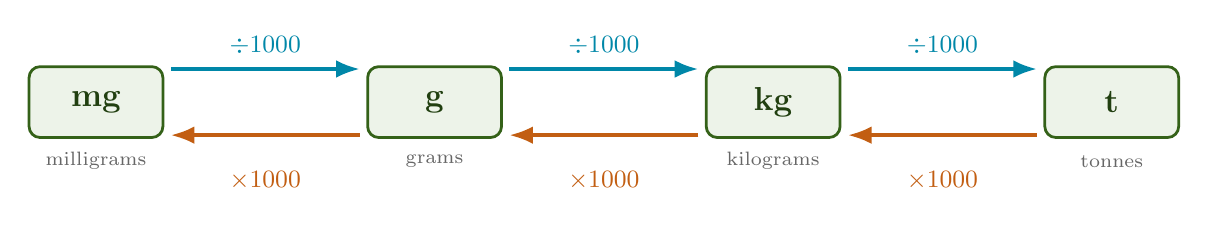
\begin{tikzpicture}[x=1cm, y=1cm, line width=1pt]
  \foreach \i/\u/\w in {0/mg/milligrams, 1/g/grams, 2/kg/kilograms, 3/t/tonnes}{
    \node[draw=cbgreen!70!black, fill=cbgreen!10, rounded corners=4pt,
          minimum width=1.7cm, minimum height=0.9cm,
          font=\large\bfseries, text=cbgreen!45!black] (n\i) at (\i*4.3,0) {\u};
    \node[font=\scriptsize, text=black!60] at (\i*4.3,-0.75) {\w};}
  \foreach \i in {0,1,2}{
    \draw[cbteal, -{Latex[length=3mm]}, line width=1.3pt]
      ({\i*4.3+0.95},0.42) -- ({\i*4.3+3.35},0.42);
    \node[above, font=\small, text=cbteal] at ({\i*4.3+2.15},0.46) {$\div 1000$};
    \draw[cborange, -{Latex[length=3mm]}, line width=1.3pt]
      ({\i*4.3+3.35},-0.42) -- ({\i*4.3+0.95},-0.42);
    \node[below=10pt, font=\small, text=cborange] at ({\i*4.3+2.15},-0.40)
      {$\times 1000$};}
\end{tikzpicture}
\end{center}

% -- X17 --------------------------------------------------------------------
\qhead[cbgreen]{X17}{One step}

\noindent Use the ladder. Each of these is \textbf{one} step.

\vspace{4pt}
\begin{multicols}{2}
\begin{enumerate}[label=(\alph*), itemsep=11pt]
  \item $5 \; \mathrm{kg} = \blank[2.2cm] \; \mathrm{g}$
  \item $2000 \; \mathrm{mg} = \blank[2.2cm] \; \mathrm{g}$
  \item $0.4 \; \mathrm{t} = \blank[2.2cm] \; \mathrm{kg}$
  \item $750 \; \mathrm{g} = \blank[2.2cm] \; \mathrm{kg}$
  \item $1.8 \; \mathrm{g} = \blank[2.2cm] \; \mathrm{mg}$
  \item $60 \; \mathrm{kg} = \blank[2.2cm] \; \mathrm{t}$
\end{enumerate}
\end{multicols}

% -- X18 --------------------------------------------------------------------
\qhead[cbgreen]{X18}{Two steps}

\begin{remember}[Two steps is $\times 1000$ twice]
  kg to mg goes \key{kg $\rightarrow$ g $\rightarrow$ mg}: $\times 1000$, then
  $\times 1000$ again. That is $\times 10^6$ --- the digits move \key{six} places.

  \smallskip
  \hspace*{1.2em}$4 \; \mathrm{kg} = 4000 \; \mathrm{g} = \mathbf{4\,000\,000} \;
  \mathrm{mg}$
\end{remember}

\vspace{2pt}
\begin{multicols}{2}
\begin{enumerate}[label=(\alph*), itemsep=11pt]
  \item $3 \; \mathrm{kg} = \blank[2.6cm] \; \mathrm{mg}$
  \item $2 \; \mathrm{t} = \blank[2.6cm] \; \mathrm{g}$
  \item $500\,000 \; \mathrm{mg} = \blank[2.6cm] \; \mathrm{kg}$
  \item $0.25 \; \mathrm{t} = \blank[2.6cm] \; \mathrm{g}$
\end{enumerate}
\end{multicols}

% -- X19 --------------------------------------------------------------------
\qhead[cbgreen]{X19}{Which is heavier?}

\noindent You cannot compare two numbers until they are in the \textbf{same unit}.
Change one of them, then write $<$ or $>$.

\vspace{4pt}
\begin{enumerate}[label=(\alph*), itemsep=10pt]
  \item $400 \; \mathrm{g}$ \quad or \quad $0.5 \; \mathrm{kg}$ \; ?
        \hfill same unit: \blank[3.0cm] \quad $\nbox$
  \item $2500 \; \mathrm{mg}$ \quad or \quad $2 \; \mathrm{g}$ \; ?
        \hfill same unit: \blank[3.0cm] \quad $\nbox$
  \item $0.9 \; \mathrm{t}$ \quad or \quad $950 \; \mathrm{kg}$ \; ?
        \hfill same unit: \blank[3.0cm] \quad $\nbox$
\end{enumerate}

% -- X20 --------------------------------------------------------------------
\qhead[cbgreen]{X20}{Mr Bowen's homework}

\noindent Only \textbf{one} of these six is right. Find it, and correct the other five.

\vspace{4pt}
\begin{multicols}{2}
\begin{enumerate}[label=(\alph*), itemsep=12pt]
  \item $4.6 \times 100 = 4.600$ \; \blank[2.6cm]
  \item $7 \div 100 = 0.7$ \; \blank[2.6cm]
  \item $0.96$ to 1 d.p. $= 1.0$ \; \blank[2.6cm]
  \item $130.4$ has 4 d.p. \; \blank[2.6cm]
  \item $3 \; \mathrm{kg} = 3000 \; \mathrm{mg}$ \; \blank[2.6cm]
  \item $0.65 > 0.7$ \; \blank[2.6cm]
\end{enumerate}
\end{multicols}

% -- X21 --------------------------------------------------------------------
% The sheet in miniature, and the last question on purpose: one pair of digits
% standing in three places, then rounded.
\qhead[cbgreen]{X21}{The whole sheet in one question}

\noindent Mr Bowen's medicine bottle says \textbf{0.045 kg}.

\vspace{4pt}
\begin{enumerate}[label=(\alph*), itemsep=10pt]
  \item Write that mass in \textbf{grams}. \hfill \blank[3.4cm]
  \item Write it in \textbf{milligrams}. \hfill \blank[3.4cm]
  \item Round your \textbf{gram} answer to \textbf{1 decimal place}.
        \hfill \blank[3.4cm]
\end{enumerate}

\vspace{2pt}
\noindent Show the steps of the ladder here.

\begin{workspace}[3.2cm]\end{workspace}

\vspace{1pt}
\noindent \textbf{(d)} The digits \textbf{4} and \textbf{5} are in all three of your
answers, and nothing else about them is the same. Say in one or two sentences what
changed.

\qlines{4}

% ===========================================================================
% ANSWER KEY -- TEACHER COPY ONLY
% ===========================================================================
\ifkey
\clearpage

\hwsection[cbred]{Answer Key --- Teacher Copy}

\linespread{1.0}\selectfont
\setlist[enumerate]{itemsep=2pt, topsep=3pt, leftmargin=*}
\setlist[itemize]{itemsep=2pt, topsep=3pt, leftmargin=*}

\qhead[cbred]{X1}{One digit per column}
\noindent $6.85$: \; 6 in ones, 8 in tenths, 5 in hundredths. \\
$130.06$: \; 1 in hundreds, 3 in tens, 0 in ones, 0 in tenths, 6 in hundredths. \\
$0.904$: \; 0 in ones, 9 in tenths, 0 in hundredths, 4 in thousandths.

\smallskip
\noindent{\small \textbf{$130.06$ is the row that does the work}, and the two zeros are
why it is on the sheet. The 0 in the ones column and the 0 in the tenths column are
both \emph{holding a place open}. A student who leaves them out writes $13.6$ and has
changed the number by more than a hundred. \\
$0.904$ traps the other way: there is nothing in front of the point, and students write
$904$ or leave the ones column blank. The 0 in the ones is written, and the table has a
column for it.}

\qhead[cbred]{X2}{The same digit, five different jobs}
\noindent 1 \textbf{C} \sep 2 \textbf{A} \sep 3 \textbf{B} \sep 4 \textbf{E} \sep
5 \textbf{D}

\smallskip
\noindent{\small 2 and 3 are the pair to mark together: $0.63$ and $0.86$ both have a
6 after the point, and it is worth ten times more in one than the other. Nothing about
the digit says which --- only the column does. \\
5 is the one students skip, because the 6 is in front of the point and they have decided
the question is about decimals.}

\qhead[cbred]{X3}{Saying it out loud}
\noindent $5.9$ five point nine \sep $0.71$ nought point seven one \sep
$8.06$ eight point zero six \\
three point one four is $3.14$ \sep twenty point zero five is $20.05$

\smallskip
\noindent{\small \textbf{This is the listening question and it is worth doing out loud
with the class.} ``Twelve point thirty-four'' is what almost everyone says first, and it
is wrong in a way that matters: ``point thirty-four'' would have to mean the tens column
after the point, and there is no such column. \\
$8.06$ and $20.05$ are the two that decide it. A student who writes $8.6$ from ``eight
point zero six'' has not heard the zero, and a student who says ``eight point six'' for
$8.06$ has not read it. Same error, two directions. \\
Accept ``zero'' or ``nought'' for 0. Do not accept ``oh'' in written work.}

\qhead[cbred]{X4}{Which is bigger?}
\noindent (a) $>$ \quad (b) $<$ \quad (c) $>$ \quad (d) $<$ \quad
(e) \textbf{equal} \quad (f) $>$

\smallskip
\noindent \textbf{The pair that is neither:} (e), $7.30$ and $7.3$. A zero on the
\emph{end} of a decimal adds nothing --- there are three tenths and no hundredths either
way.

\smallskip
\noindent{\small (a), (c) and (f) are all the same question: the longer number is the
smaller one. Students compare digit counts instead of comparing tenths. \\
(d) is the hardest, because $0.09$ has a 9 in it and $0.1$ has a 1, and 9 is bigger than
1. It is in the \emph{hundredths} column, so it is worth less. Send them to the table in
X1. \\
(e) is the one that matters for Part 3. A trailing zero changes nothing about the
\emph{size} of a number --- which is exactly why X15's $35.0$ is not about size. It is
about saying how exact you were.}

\qhead[cbred]{X5}{Watch it happen}
\noindent Row 2 is $46 \cdot$ (4 in tens, 6 in ones); row 3 is $460 \cdot$ (4 in
hundreds, 6 in tens, 0 in ones). \\
\textbf{(a)} $4.6$, $46$, $460$. \\
\textbf{(b)} The \textbf{digits} moved, one column to the left each time. The
\textbf{point} stayed where it was.

\smallskip
\noindent{\small \textbf{(b) is the sheet.} If a student can write that sentence, the
rest of Part 2 is bookkeeping. If they cannot, no amount of practice at X6 will help,
because they are still adding zeros. \\
Row 3 needs a 0 written in the ones column. It is the first time on the sheet that a
zero has to be invented rather than copied, and it is the same zero as $7 \div 100 =
0.07$ in X7.}

\qhead[cbred]{X6}{Multiplying moves the digits left}
\noindent (a) $32$ \quad (b) $7$ \quad (c) $54.8$ \quad (d) $320$ \quad (e) $70$ \quad
(f) $690$ \\
(g) $3200$ \quad (h) $5$ \quad (i) $1280$

\smallskip
\noindent{\small (b) and (h) are the two that look wrong to a student: $0.7 \times 10$
is $7$, with nothing after the point at all, and $0.05 \times 100$ is $5$. Multiplying
made the point disappear. It did not --- the digits walked past it. \\
(a), (d) and (g) are deliberately the same digits three times. Point at the column.}

\qhead[cbred]{X7}{Dividing moves the digits right}
\noindent (a) $4.6$ \quad (b) $0.8$ \quad (c) $52$ \quad (d) $0.46$ \quad (e) $0.08$
\quad (f) $5.2$ \\
(g) $0.046$ \quad (h) $0.009$ \quad (i) $0.035$

\smallskip
\noindent{\small (e), (g), (h) and (i) are the whole point of the question: a zero has
to be \emph{written} where nothing landed. Expect $0.8$ for (e), $0.46$ for (g) and
$0.9$ for (h) --- in each case the student moved the right number of places and then
declined to write the zeros that prove it. \\
(i) is the hardest item on the sheet: $3.5$ already has a decimal point, and the digits
still move two places right. $3.5 \rightarrow 0.35 \rightarrow 0.035$.}

\qhead[cbred]{X8}{The little raised number}
\noindent $10^3 = 1000$, ten cubed \sep $10^5 = 100\,000$, ten to the power of five
\sep $10^4 = 10\,000$, ten to the power of four

\smallskip
\noindent{\small The third column is the question. ``Squared'' and ``cubed'' are not
optional vocabulary --- they are how the exam paper says $10^2$ and $10^3$, and from
$10^4$ upwards English switches to ``to the power of''. Make them say all four aloud. \\
The last row runs backwards, from the written-out number to the power. Students count
the digits (5) instead of the zeros (4).}

\qhead[cbred]{X9}{Now with the power written in}
\noindent (a) $240$ \quad (b) $60$ \quad (c) $150\,000$ \quad (d) $8.3$ \quad
(e) $0.006$ \quad (f) $0.25$

\smallskip
\noindent{\small (b) is the one to watch: $0.06 \times 10^3$ is $60$, and it is a jump
of three columns straight through the point. Expect $0.06000$ from anyone still adding
zeros, and $6$ from anyone who moved two. \\
(f) is $10^1$, which the class has probably not seen written down. It is just 10. Say
so; do not make a lesson of it.}

\qhead[cbred]{X10}{Which way, and how far?}
\noindent $6.1 \rightarrow 0.061$: \; right, 2, $\div 10^2$ \\
$90 \rightarrow 9000$: \; left, 2, $\times 10^2$ \\
$7 \rightarrow 0.7$: \; right, 1, $\div 10^1$ (or $\div 10$)

\smallskip
\noindent{\small This is X6 to X9 read backwards, and it is the question that shows
whether a student is counting columns or guessing. \\
The first row is the one that goes wrong. $6.1$ to $0.061$ looks like ``two zeros
appeared'', so students write 3. Make them put both numbers in a place-value table and
count where the 6 went: ones to hundredths is two columns.}

\qhead[cbred]{X11}{Which end is it nearer?}
\noindent (a) $\mathbf{3.4}$ \quad (b) $\mathbf{3.7}$ \quad (c) nearer \textbf{3}
\quad (d) nearer \textbf{4}

\smallskip
\noindent{\small The whole of X12 is on this picture, and it is worth saying so out
loud: rounding is not a rule about the digit 5, it is a question about which end of the
line you are nearer, and the digit is just the quick way to answer it. \\
If a student gets (c) or (d) wrong, they are reading the marks rather than the
distances. Put a finger on P and walk it both ways.}

\qhead[cbred]{X12}{Round to the nearest whole number}
\noindent (a) $6$ \quad (b) $9$ \quad (c) $15$ \quad (d) $0$ \quad (e) $30$ \quad
(f) $1$

\smallskip
\noindent{\small (d) is the item that gets left blank: $0.4$ rounds to \textbf{0}, and
students do not believe zero is an answer. \\
(e) is the carry --- $29.8$ goes to $30$, not $29$ and not $20$. \\
(c) is the exactly-halfway convention. $14.5$ rounds \emph{up} because that is the rule,
not because 15 is nearer; 14 and 15 are the same distance away. Say that once.}

\qhead[cbred]{X13}{Counting decimal places}
\noindent $5.28$: 2 \sep $0.9$: 1 \sep $12.346$: 3 \sep $130.4$: 1 \sep
$7.0625$: 4 \sep $86$: \textbf{0}

\smallskip
\noindent{\small $130.4$ is the trap and it is the reason the question exists: students
count \emph{all} the digits, or count from the front, and answer 4. Decimal places are
counted from the point, rightwards, and there is one. \\
$86$ has \textbf{no} decimal places. Several will leave it blank.}

\qhead[cbred]{X14}{Round to 1 decimal place}
\noindent (a) $4.6$ \quad (b) $8.2$ \quad (c) $0.3$ \quad (d) $23.8$ \quad (e) $9.4$
\quad (f) $0.3$

\smallskip
\noindent{\small (c) and (f) both have a \emph{third} decimal, and it is there to be
ignored. Rounding to 1 d.p. looks at the second digit only: $0.348$ is $0.3$, not $0.35$
and not $0.4$. A student who rounds $0.348$ to $0.35$ and then to $0.4$ has rounded
twice, which is the error E3 on the main packet is built on. \\
(b) is the carry within the decimals: $8.17$ goes to $8.2$.}

\qhead[cbred]{X15}{The zero that has to stay}
\noindent (a) $\mathbf{7.0}$ \quad (b) $\mathbf{1.0}$ \quad (c) $\mathbf{20.0}$ \quad
(d) $\mathbf{2.0}$

\smallskip
\noindent{\small All four answers end in $.0$ and the instruction line says so, which
turns this from a trick into a drill. Anyone who writes 7, 1, 20 and 2 has understood
the arithmetic perfectly and lost every mark, and that is worth saying plainly. \\
(b) is the biggest jump: $0.96$ becomes $1.0$, and the number in front of the point
changes from 0 to 1. \\
This is the same fact as X4(e) turned around. There, the trailing zero added nothing to
the \emph{size}. Here it adds nothing to the size either --- what it adds is the
statement \emph{I rounded this to one place}, which is what the question asked for.}

\qhead[cbred]{X16}{Round to 2 decimal places}
\noindent (a) $3.47$ \quad (b) $0.18$ \quad (c) $12.01$ \quad (d) $\mathbf{9.00}$

\smallskip
\noindent{\small (d) is the hardest item in Part 3: $8.996$ carries through both
decimals and into the ones, and the answer is $9.00$ --- a number that looks nothing
like the question. Expect $8.99$, $9$ and $9.0$; only $9.00$ is right. \\
(c) is the other carry: the 5 rounds the second 0 up to 1.}

\qhead[cbred]{X17}{One step}
\noindent (a) $5000$ g \quad (b) $2$ g \quad (c) $400$ kg \quad (d) $0.75$ kg \quad
(e) $1800$ mg \quad (f) $0.06$ t

\smallskip
\noindent{\small (d) and (f) go \emph{up} the ladder into a number smaller than 1, which
is the direction nobody practises. Expect $750\,000$ for (d) and $60\,000$ for (f) ---
the student used the ladder and went the wrong way along it. \\
Ask which way before asking how far. Going up towards tonnes, the number gets smaller;
going down towards milligrams, it gets bigger. That is one sentence and it fixes most of
this question.}

\qhead[cbred]{X18}{Two steps}
\noindent (a) $3\,000\,000$ mg \quad (b) $2\,000\,000$ g \quad (c) $0.5$ kg \quad
(d) $250\,000$ g

\smallskip
\noindent{\small A student who writes $3000$ for (a) has taken one step and stopped, and
that is the only error worth naming here. Make them say ``kg, g, mg'' out loud and count
\emph{two} arrows before they write anything. \\
(d) has a decimal going down the ladder: $0.25$ t is $250$ kg is $250\,000$ g. The point
disappears on the first step, which students distrust --- it is X6(h) again.}

\qhead[cbred]{X19}{Which is heavier?}
\noindent (a) $0.5$ kg is $500$ g, so $400 < 500$: the \textbf{0.5 kg} is heavier. \\
(b) $2$ g is $2000$ mg, so $2500 > 2000$: the \textbf{2500 mg} is heavier. \\
(c) $0.9$ t is $900$ kg, so $900 < 950$: the \textbf{950 kg} is heavier.

\smallskip
\noindent{\small Either unit is fine as the common one --- accept $400$ g against $500$
g or $0.4$ kg against $0.5$ kg. What is not fine is comparing 400 with 0.5 and
announcing that 400 is bigger, which is what happens if the conversion is skipped, and
which gets (a) and (c) wrong together. \\
(b) is the one where skipping the conversion accidentally gives the right answer. Do not
let it pass: ask for the working.}

\qhead[cbred]{X20}{Mr Bowen's homework}
\noindent (a) \textbf{wrong} --- $460$. The digits move two columns left; you do not
write zeros on the end of a decimal. \\
(b) \textbf{wrong} --- $0.07$. Two places right from 7, and both empty columns have to
be written as zeros. \\
(c) \textbf{right.} \\
(d) \textbf{wrong} --- $130.4$ has \textbf{1} decimal place. Count from the point, not
from the front of the number. \\
(e) \textbf{wrong} --- $3\,000\,000$ mg. kg to mg is \emph{two} steps, not one. \\
(f) \textbf{wrong} --- $0.65 < 0.7$. Six tenths against seven tenths.

\smallskip
\noindent{\small One trap each from X6, X7, X15, X13, X18 and X4, in that order, which
makes this a five-minute diagnosis of the whole sheet. Whichever one a student gets
wrong, send them back to that question rather than explaining it again. \\
The instruction says one of the six is right. A student who corrects all six has not
read it, and a student who corrects none has decided Mr Bowen is reliable. \\
(c) is the right one on purpose: it is the answer that \emph{looks} wrong, because 1.0
looks like it should just be 1. That is X15, and it is the habit most likely to have
slipped back.}

\qhead[cbred]{X21}{The whole sheet in one question}
\noindent (a) $\mathbf{45}$ g \quad (b) $\mathbf{45\,000}$ mg \quad
(c) $\mathbf{45.0}$ g \\
(d) Nothing changed about the digits. Only \textbf{where the point is} --- and so which
column each digit is standing in.

\smallskip
\noindent{\small (a) is three places left, and the leading zero goes: $0.045 \rightarrow
0.45 \rightarrow 4.5 \rightarrow 45$. Expect $0.045000$ and $45\,000$. \\
(c) is the question inside the question. $45$ has no decimal places, so rounding it to 1
d.p. gives $\mathbf{45.0}$ --- a trailing zero on a number that never had a decimal part
at all. It is X15 with the carry taken away, and it is the last thing on the sheet on
purpose. \\
(d) has no single right wording. Accept anything that says the digits stayed and the
point moved --- or, better, that the \emph{digits} moved and the \emph{point} stayed,
which is what the cover claims and what X5(b) asked for. Both sentences describe the
same thing and a student who can argue for either has understood it.}

\fi
\end{document}
